\documentclass{article}
\title{Sprawozdanie 2 \\ Testowanie opracowanej metody heurystycznej}
\date{2018-06-01}
\author{Mateusz Babiaczyk, Bartosz Nawrotek}
\usepackage[utf8]{inputenc}
\usepackage[T1]{fontenc}
\usepackage{graphicx}
\usepackage{float}
\graphicspath{ {Wykresy/} }
\usepackage{geometry}
 \geometry{
 a4paper,
 total={170mm,257mm},
 left=20mm,
 top=20mm,
 }

\begin{document}
\maketitle
\section{Zmiany w algorytmie}  
Po zaimplementowaniu algorytmu i zauważeniu jego słabych osiągnięć, zdecydowano by wprowadzić zmiany w zastosowanym podejściu algorytmicznym. Poniżej w kilku sekcjach omówiono te cześci algorytmu, które zostały zastąpione.
\subsection{Kodowanie}
Zmiana w kodowaniu polega na traktowaniu osobnika jako cykliczny, spowodowało to że każdy osobnik jest zbiórem rozwiązań z przesuniętym początkiem o jeden oligonukleotyd. Nie pogorszyło to złożoności obliczeniowej wyznaczania funkcji celu, która pozostała równa $O(n)$, gdzie $n$ jest długością osobnika. Pozwoliło natomiast na traktowanie jednego rozwiązania jako zbioru $n$ różnych rozwiązań i korzystania z tej części osobnika o najlepszym przystosowaniu.
\subsection{Mutacje}
W funkcji odpowiedzialnej za dokonanie mutacji osobnika została zastosowana odrębna idea ze względu na to, że rozwiązania pozostawały w minimach lokalnych. Przyjęto konwencję, w której każdy z oligonukleotydów ma wygenerowane koło fortuny. Dla koła fortuny oligonukleotydu $A$, każdy z oligonukleotydów otrzymuje wycinek koła w zależności od funkcji kosztu między nim a osobnikiem $A$ (Dla kosztu maksymalnego, nie otrzymuje wycinka). Gdy następuje mutacja osobnika wybierany jest oligoukleotyd $a$ o największym koszcie będącym sumą kosztów z sąsiednimi oligonukleotydami oraz losowany jest oligonukleotyd $b$ przy użyciu wygenerowanego koła fortuny przed którym umieszczany zostaje oligonukleotyd $a$. Dzięki temu algorytm przemieszcza oligonukleotyd o najgorszym dopasowaniu w co najmniej tak dobre miejsce preferując miejsca lepszego dopasowania.
\subsection{Krzyżowanie}
Krzyżowanie zaczyna się w dokładnie taki sam sposób jak w pierwotnym algorytmie, a mianowicie od pewnego wylosowanego przedziału przepisuje się oligonukleotydy do nowo tworzonego osobnika (kopiuje wycinek i wkleja go do nowego osobnika) z wybranego osobnika z populacji rodzicielskiej. Następnie uzupełniany jest koniec osobnika wartościami z innego osobnika z populacji rodzicielskiej, uważając oczywiście by dany oligonukleotyd nie został powtórzony. W ten sam sposób zostaje uzupełniony początek osobnika z nowej populacji. \\ Wszystkie oligonukleotydy które nie zostały dodane wstawiane są, w miejsca w których ich koszt będzie najmniejszy. Motywacją było przyspierzenie zbieżności algorytmu oraz zachowanie losowości dzięki losowemu doborowi punktów krzyżowania. Tym samy dając lepsze rozwiązania w krótszym czasie przetwarzania jak i dając możliwość na opuszczenie minimów lokalnych.
\section{Testy}
Testy wykonano na dwóch wariantach zaproponowanej hybrydy algorytmu genetycznego, jednym z nich było startowanie od losowej populacji początkowej, drugim natomiast początkowe wygenerowania jednego osobnika za pomocą algorytmu zachłannego, który ma na przyspieszyć zbierzność pozostałych rozwiązań do optimum.
Dodatkowo wybrane zostało kryterium stopu jako 200 iteracji algorytmu.
W testach mierzono upływ czasu, jak i zmiany jakości rozwiązań co 10 iteracji algorytmu, aby pokazać poprawę rozwiązań wraz z kolejnymi iteracjami. Jako jakość rozwiązania przyjęto stosunek ilości oligonukleotydów rozwiązania uzyskanego przez algorytm do ilości oligonukleotydów w rozwiązaniu optymalnym. Jakość wyrażamy w procentach.
\subsection{Wyniki algorytmu dla błędów negatywnych, losowych}
\begin{figure}[H]
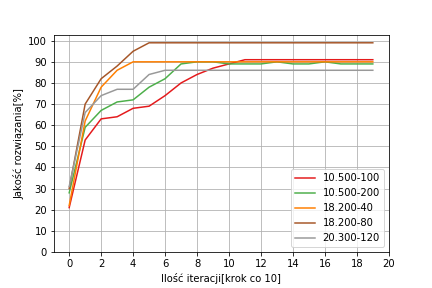
\includegraphics[width=0.5\textwidth]{neg-los1.png}
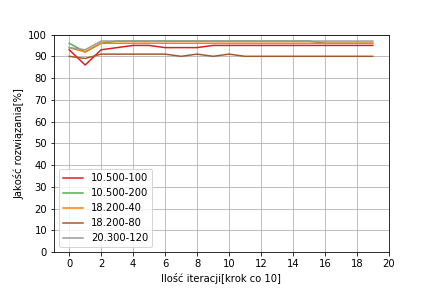
\includegraphics[width=0.5\textwidth]{neg-los-greedy1.png}
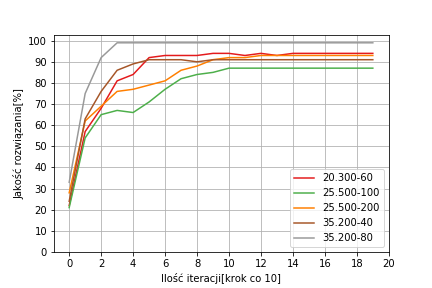
\includegraphics[width=0.5\textwidth]{neg-los2.png}
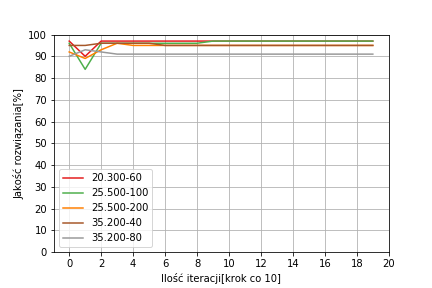
\includegraphics[width=0.5\textwidth]{neg-los-greedy2.png}
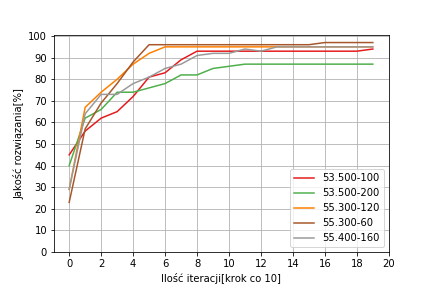
\includegraphics[width=0.5\textwidth]{neg-los3.png}
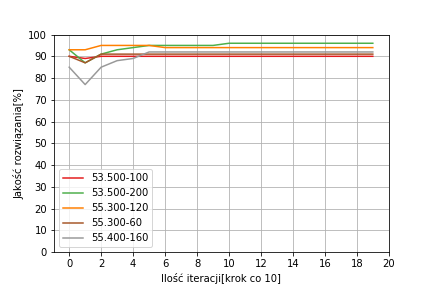
\includegraphics[width=0.5\textwidth]{neg-los-greedy3.png}
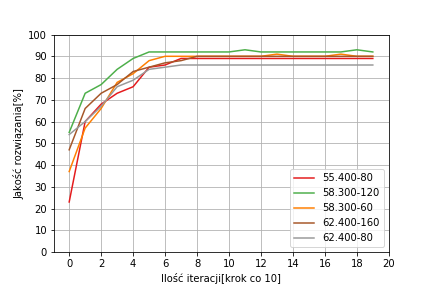
\includegraphics[width=0.5\textwidth]{neg-los4.png}
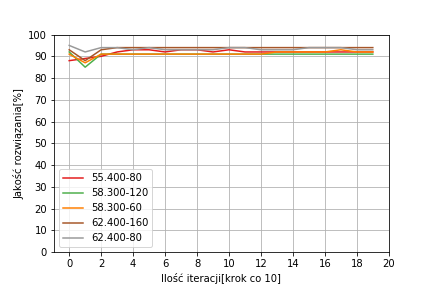
\includegraphics[width=0.5\textwidth]{neg-los-greedy4.png}
\caption{Porównanie algorytmu dla błędów negatywnych, losowych bez (po lewej stronie) oraz z wykorzystanym osobnikiem wygenerownym przez algorytm zachłanny (po prawej stronie) w zależności od ilości iteracji.}
\end{figure}
\begin{figure}[H]
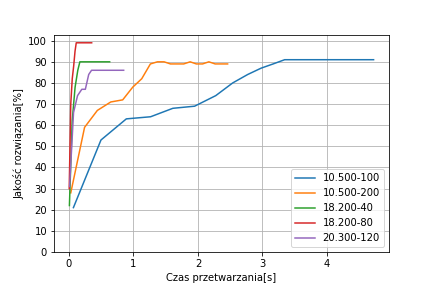
\includegraphics[width=0.5\textwidth]{Czasneg-los1.png}
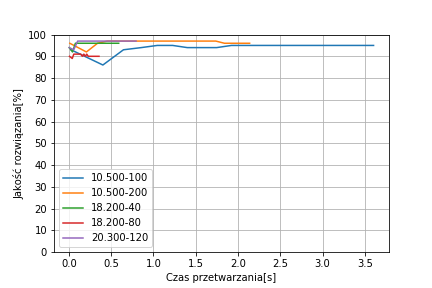
\includegraphics[width=0.5\textwidth]{Czasneg-los-greedy1.png}
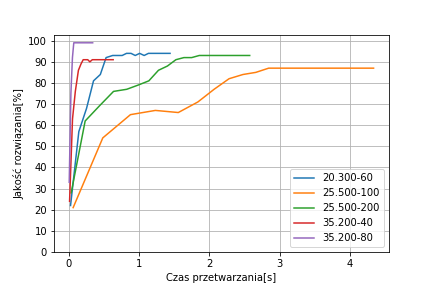
\includegraphics[width=0.5\textwidth]{Czasneg-los2.png}
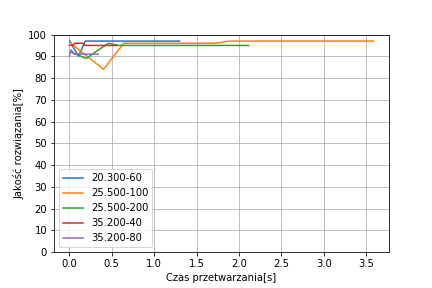
\includegraphics[width=0.5\textwidth]{Czasneg-los-greedy2.png}
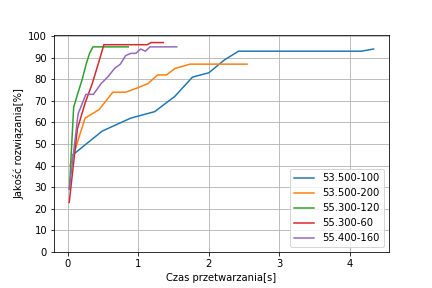
\includegraphics[width=0.5\textwidth]{Czasneg-los3.png}
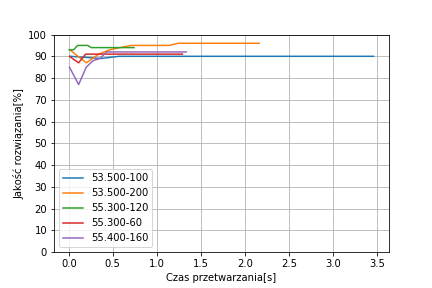
\includegraphics[width=0.5\textwidth]{Czasneg-los-greedy3.png}
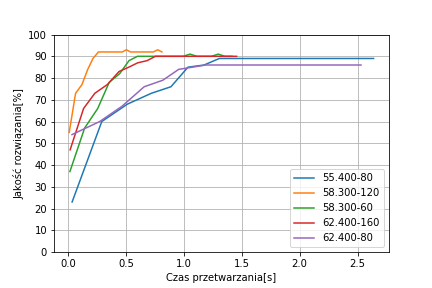
\includegraphics[width=0.5\textwidth]{Czasneg-los4.png}
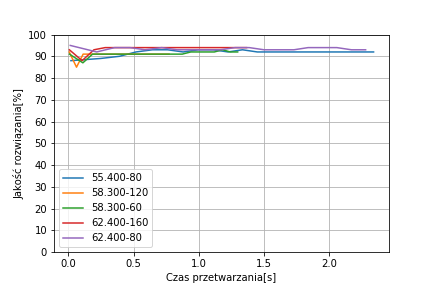
\includegraphics[width=0.5\textwidth]{Czasneg-los-greedy4.png}
\caption{Porównanie algorytmu dla błędów negatywnych, losowych bez (po lewej stronie) oraz z wykorzystanym osobnikiem wygenerownym przez algorytm zachłanny (po prawej stronie) w zależności od czasu przetwarzania}
\end{figure}
Jak widać, dla błędów negatywnych, losowych algorytm otrzymuje rozwiązanie o średniej jakości 90\%. W algorytmie z wykorzystaniem osobnika wygenerowanego przez algorytm zachłanny częściej uzyskiwane są lepsze wyniki z powodu początkowego uszeregowania które ma bardzo dobrą jakość. Rozwiązania algorytmu bez wykorzystania algorytmu zachłannego zbiegają do podobnej jakości wyników. Czasem jakość wyników jest nawet lepsza, prawdopodobnie ze względu na to, że osobniki za szybko upodabniają się do wyniku algorytmu zachłannego. Dodatkowo warto zauważyć, że wykresy po prawej stronie wskazują na polepszenie wyniku wygenerowanego przez algorytm zachłanny.
\subsection{Wyniki algorytmu dla błędów negatywnych na końcach sekwencji}
\begin{figure}[H]
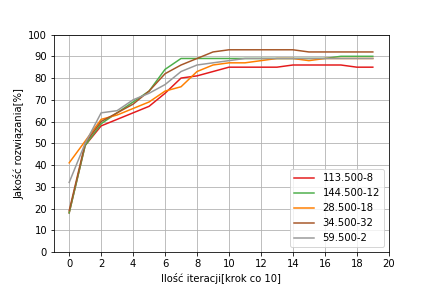
\includegraphics[width=0.5\textwidth]{neg-pow1.png}
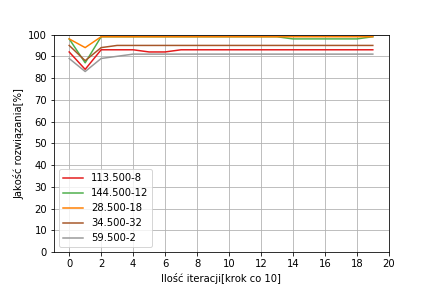
\includegraphics[width=0.5\textwidth]{neg-pow-greedy1.png}
\caption{Porównanie algorytmu dla błędów negatywnych na końcach sekwencji bez (po lewej stronie) oraz z wykorzystanym osobnikiem wygenerownym przez algorytm zachłanny (po prawej stronie) w zależności od ilości iteracji}
\end{figure}
\begin{figure}[H]
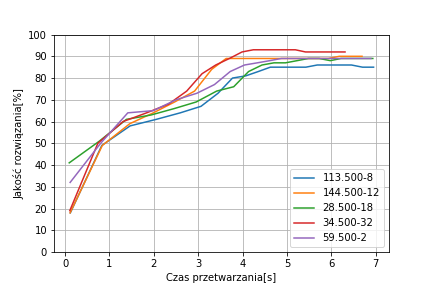
\includegraphics[width=0.5\textwidth]{Czasneg-pow1.png}
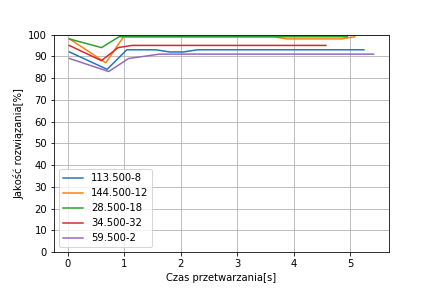
\includegraphics[width=0.5\textwidth]{Czasneg-pow-greedy1.png}
\caption{Porównanie algorytmu dla błędów negatywnych na końcach sekwencji bez (po lewej stronie) oraz z wykorzystanym osobnikiem wygenerownym przez algorytm zachłanny (po prawej stronie) w zależności od czasu przetwarzania}
\end{figure}
W przypadku błędów negatywnych na końcach sekwencji wyniki są zbliżone do wyników błędów negatywnych losowych. Różnicą jest fakt, że przy rozpoczęciu od wygenerowania losowej populacji początkowej zbieganie trwa dłużej.
\subsection{Wyniki algorytmu dla błędów pozytywnych, losowych}
\begin{figure}[H]
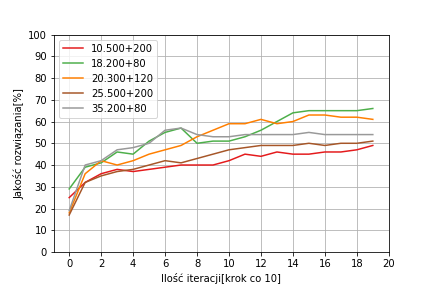
\includegraphics[width=0.5\textwidth]{poz-los1.png}
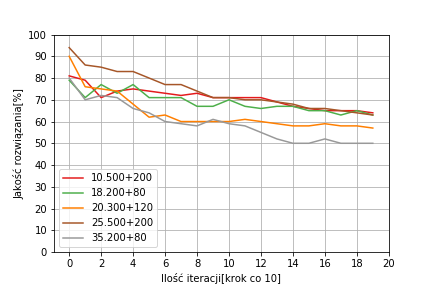
\includegraphics[width=0.5\textwidth]{poz-los-greedy1.png}
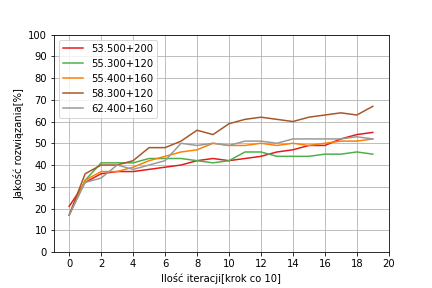
\includegraphics[width=0.5\textwidth]{poz-los2.png}
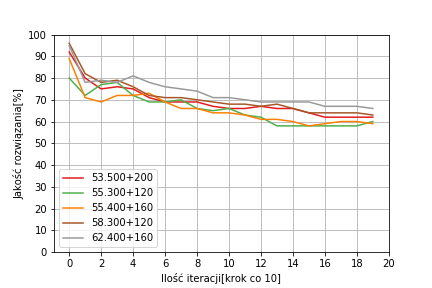
\includegraphics[width=0.5\textwidth]{poz-los-greedy2.png}
\caption{Porównanie algorytmu dla błędów pozytywnych, losowych bez (po lewej stronie) oraz z wykorzystanym osobnikiem wygenerownym przez algorytm zachłanny (po prawej stronie) w zależności od ilości iteracji}
\end{figure}
\begin{figure}[H]
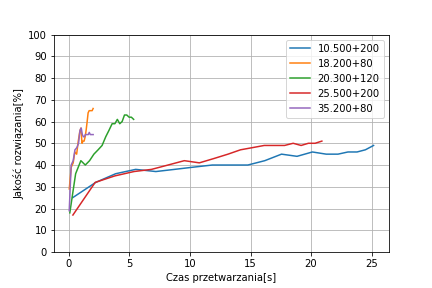
\includegraphics[width=0.5\textwidth]{Czaspoz-los1.png}
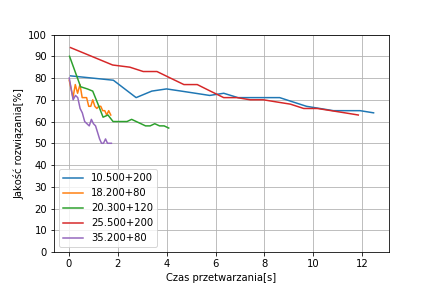
\includegraphics[width=0.5\textwidth]{Czaspoz-los-greedy1.png}
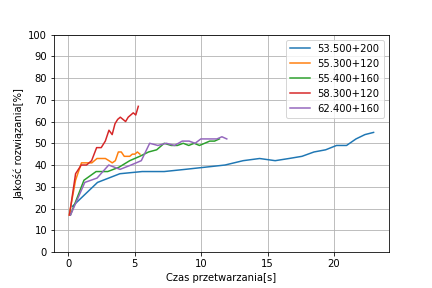
\includegraphics[width=0.5\textwidth]{Czaspoz-los2.png}
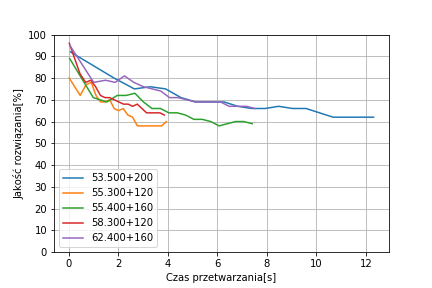
\includegraphics[width=0.5\textwidth]{Czaspoz-los-greedy2.png}
\caption{Porównanie algorytmu dla błędów pozytywnych, losowych bez (po lewej stronie) oraz z wykorzystanym osobnikiem wygenerownym przez algorytm zachłanny (po prawej stronie) w zależności od czasu przetwarzania}
\end{figure}
Dla błędów pozytywnych losowych algorytm uzyskuje średnie wyniki w okolicach 60\%. Dodatkowo algorytm z początkiem zachłannym tylko pogarsza swoje wyniki po lepszym wyniku zachłannym, żeby ostatecznie dojść do prawie tak samo dobrego wyniku jak algorytm bez początku zachłannego. Jest to związane z przyjęciem w metodzie mutacji kryterium wyboru oligonukleotydu na podstawie najsłabszego dopasowania. Powodem pogarszania wyniku jest fakt, że w przypadku błędów pozytywnych często wiąrze się to z wyborem oligonukleotydu będącego tym, nie występującym w oryginalnej sekwencji.
\subsection{Wyniki algorytmu dla błędów pozytywnych, na końcach sekwencji}
\begin{figure}[H]
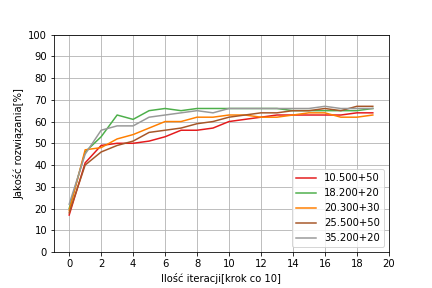
\includegraphics[width=0.5\textwidth]{poz-oli1.png}
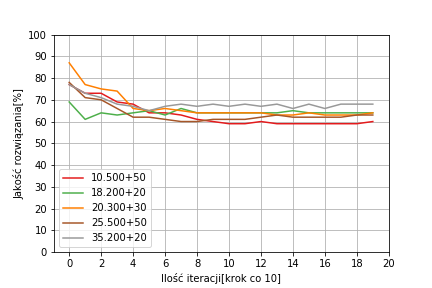
\includegraphics[width=0.5\textwidth]{poz-oli-greedy1.png}
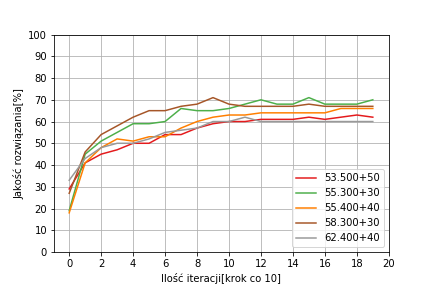
\includegraphics[width=0.5\textwidth]{poz-oli2.png}
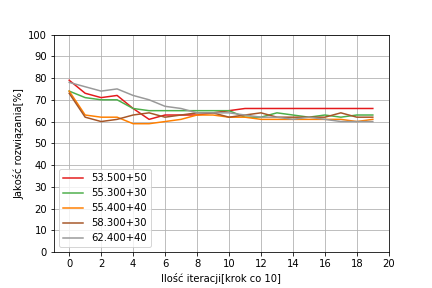
\includegraphics[width=0.5\textwidth]{poz-oli-greedy2.png}
\caption{Porównanie algorytmu dla błędów pozytywnych na końcach sekwencji bez (po lewej stronie) oraz z wykorzystanym osobnikiem wygenerownym przez algorytm zachłanny (po prawej stronie) w zależności od ilości iteracji}
\end{figure}
\begin{figure}[H]
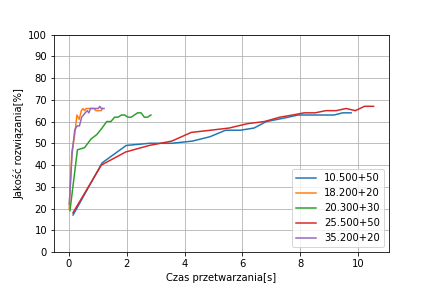
\includegraphics[width=0.5\textwidth]{Czaspoz-oli1.png}
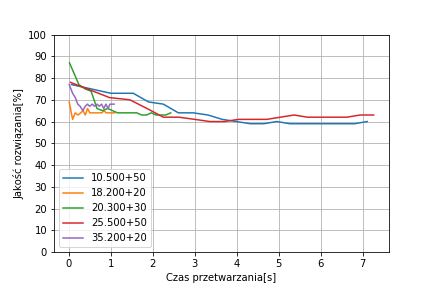
\includegraphics[width=0.5\textwidth]{Czaspoz-oli-greedy1.png}
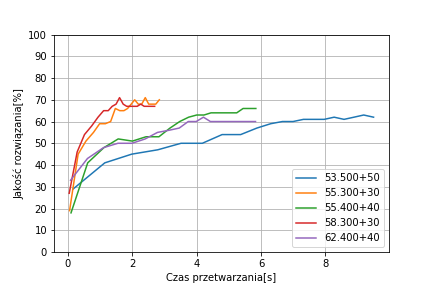
\includegraphics[width=0.5\textwidth]{Czaspoz-oli2.png}
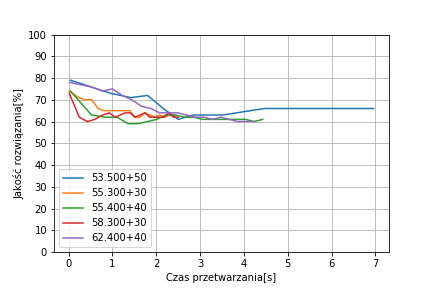
\includegraphics[width=0.5\textwidth]{Czaspoz-oli-greedy2.png}
\caption{Porównanie algorytmu dla błędów pozytywnych na końcach sekwencji bez (po lewej stronie) oraz z wykorzystanym osobnikiem wygenerownym przez algorytm zachłanny (po prawej stronie) w zależności od czasu przetwarzania}
\end{figure}
Ostatnią kategorią są błędy pozytywne z przekłamaniami na końcach oligonukleotydów. Jak widać radzi on sobie odrobinę lepiej niż dla błędów pozytywnych losowych, dodatkowo algorytm z rozpoczęciem zachłannym nie pogarsza tak mocno rozwiązań (algorytm zachłanny ma większe problemy z optymalnym ustawieniem i jego wykonanie nie powoduje od razu ustawienia pierwszej iteracji na wysokości 90-95\%, a nieco niżej na 70-80\%).
\section{Wnioski}
Zaproponowana hybryda algorytmu genetycznego wykazuje lepsze działanie w przypadku występowania błędów negatywnych. Początkowe pogorszenie rozwiązań w przypadku korzystania z rozwiązania wygenerowanego przez algorytm zachłanny wynika z zastosowania wymienionej metody mutacji, jak i z faktu, że do populacji początkowej dołączany jest tylko jeden osobnik wygenerowany przez algorytm zachłanny. O ile w przypadku błędów pozytywnych następuje szybka poprawa rozwiązania, o tyle własności błędów negatywnych nie pozwalają na poprawę rozwiązań przez przyjętą metodę mutacji, a krzyżowanie nie jest w stanie sprawić, że rozwiązanie wyjdzie z optimum lokalnego. Dodatkowo można wyciągnąć wniosek, że klasyczny algorytm genetyczny nie nadaje się do rozwiązywania problemu sekwencjonowania DNA ze względu na to, że jest to problem, w którym jest bardzo niskie prawdopodobieństwo na wylosowanie ułożenia oligonukleotydów w optymalny sposób. Kluczowe więc jest odpowiednie dokonanie modyfikacji poszczególnych  założeń klasycznego algorytmu genetycznego w celu przyspieszenia zbiegania rozwiązań do optimum. W wypadku prezentowanej metody ukazały się jej zarówno mocne, jak i słabe strony, które skłaniają do kolejnej modyfikacji załorzeń przyjętych na etapie projektowania algorytmu. Propozycją modyfikacji, jest umożliwienie odrzucenia oligonukleotydów słabo pasujących do rozwiązania w celu pozbycia się potencjalnych błędów pozytywnych. Powodowałoby to jednak konieczność przyjęcia innego kodowania rozwiązania, lub próba odmiennego jego interpretowania.
\end{document}


